\section{Weak sesion}
\paragraph{Vulnerabilidad} En esta vulnerabilidad trataremos de ver nuestra cookie 
de sesión y predecir las de los demás a partir de la secuencia que siga. De tal forma 
que probaríamos valores consecutivos de dicha secuencia hasta obtener la sesión de un usuario.
En este ejercicio trataremos de adivinar las secuencias.
\paragraph{Nivel bajo} Lo primero que debemos hacer es abrir el inspector y ver en 
la sección de {\it storage} los valores de las cookies (figura \ref{fig:weakinsp}). Como se ve en la figura 
\ref{fig:weakuno} el valor que miraremos es {\it dvwaSession}.
\begin{figure}[ht!]
    \centering
    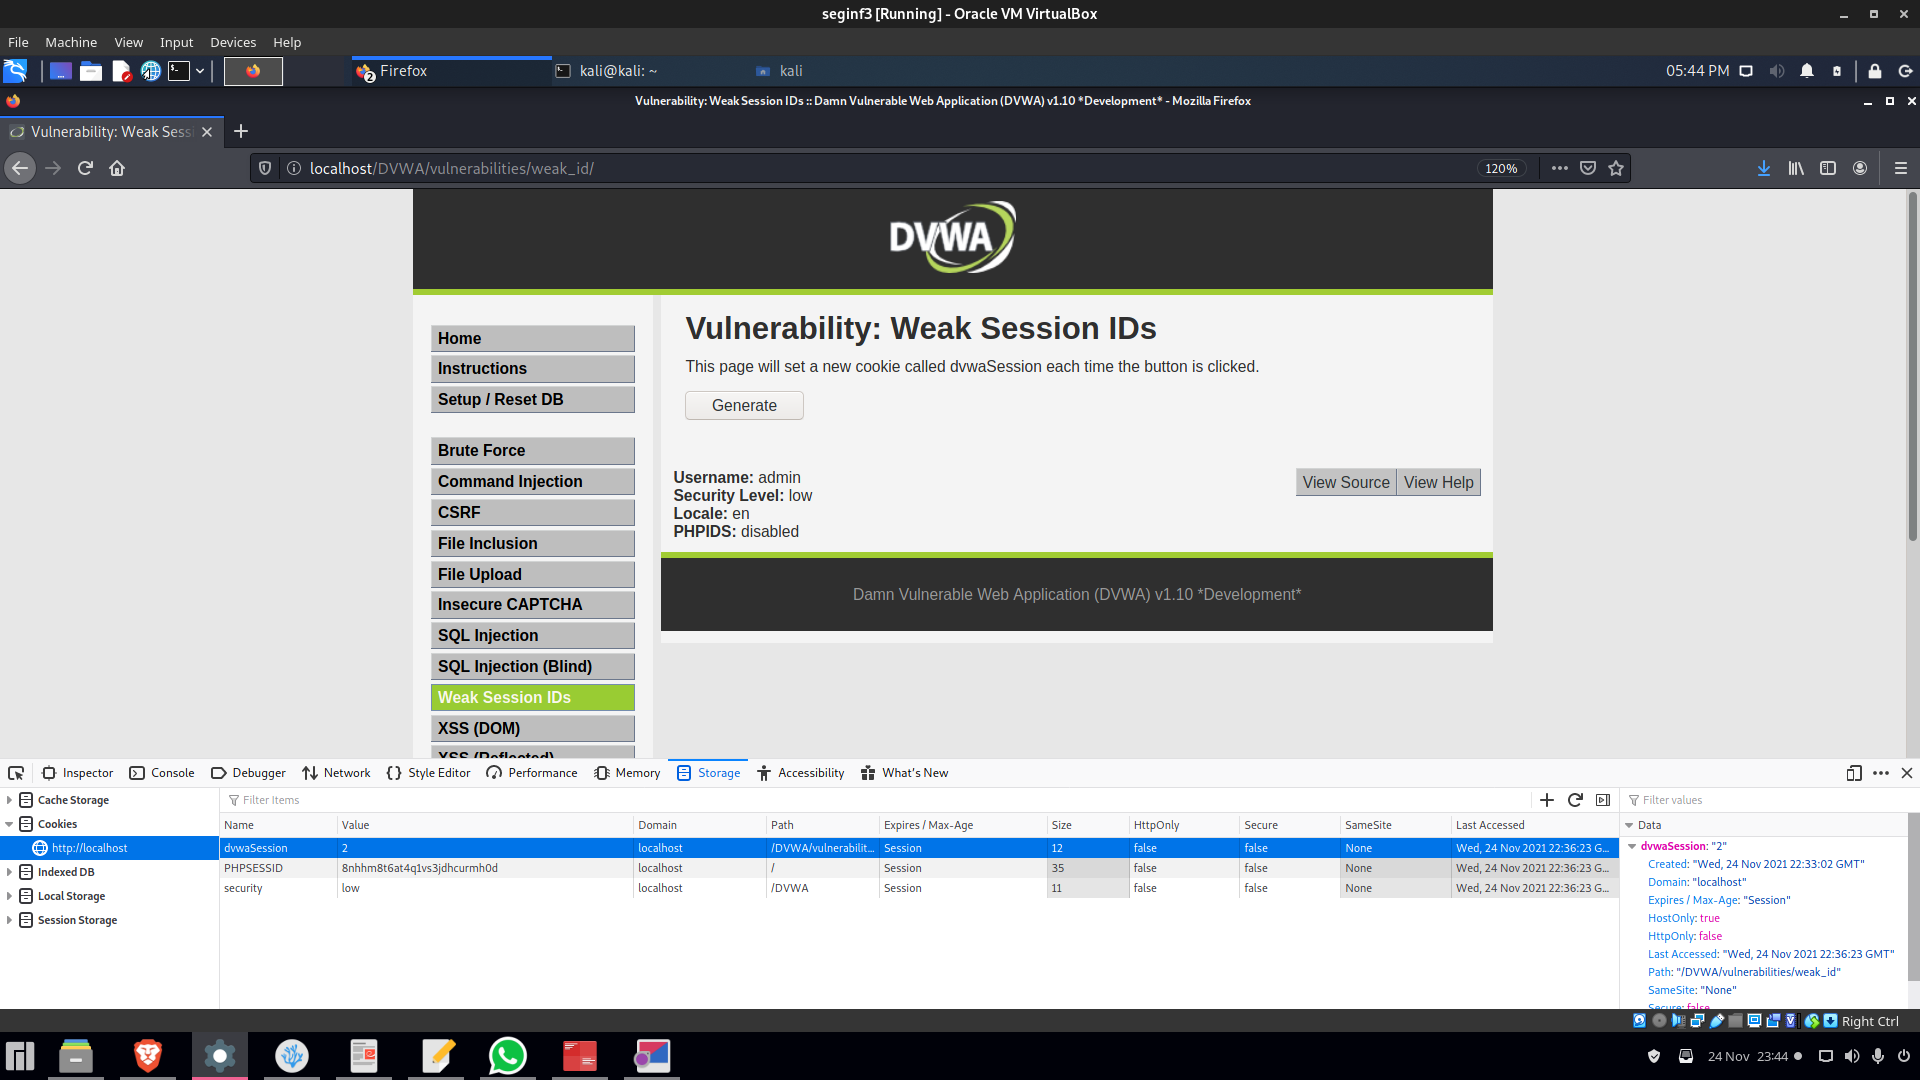
\includegraphics[width=14cm]{img/weak/inspector.png}
    \caption{Inspector del navegador}
    \label{fig:weakinsp}
\end{figure}

\begin{figure}[ht!]
    \centering
    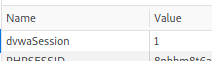
\includegraphics[width=14cm]{img/weak/one.png}
    \caption{Valor inicial }
    \label{fig:weakuno}
\end{figure}

Si volvemos a generar un id se obtiene dos y luego tres. Por lo que consideraremos que la secuencia es empezar en uno
e ir sumando el valor de uno cada vex (1,2,3,4,5,...)
\paragraph{Nivel medio}  El método es el mismo de usar el inspector del navegador, mirando los valores que adopta el id de 
sesión. Tras generar varios valores se ha obtenido:
\begin{itemize}
    \item 1637794074
    \item 1637794076
    \item 1637794077
    \item 1637794080
\end{itemize}

 Lo primero que se aprecia es que son valores 
muy similares, solo que en vez de aumentar de uno en uno aumenta entre 1 y 3 dependiendo el caso. No supimos sacar la sucesión, 
pero mirando el código fuente nos dimos cuenta que es el tiempo en segundos desde el 1 de enero de 1970. Por lo que si queremos saber la 
cookie de un usuario tendríamos que saber cuando se conecto al sistema y recordemos que esto se puede obtener mediante el {\it command injection} con el comando {\it who}.
